% \Image{Capa do livro (; )}{PNLD2022-001-01.png}
% \Image{Ilustração do livro (Acorde/Manuella Silveira; Acorde)}{PNLD2022-001-04.png}
% \Image{Ilustração do livro (Acorde/Manuella Silveira; Acorde)}{PNLD2022-001-05.png}
% \Image{Ilustração do livro (Acorde/Manuella Silveira; Acorde)}{PNLD2022-001-06.png}

\documentclass[11pt]{extarticle}
\usepackage{manualdoprofessor}
\usepackage{fichatecnica}
\usepackage{lipsum,media9}
\usepackage[justification=raggedright]{caption}
\usepackage[one]{bncc}
\usepackage[acorde]{../edlab}
\usepackage{marginnote}
\usepackage{pdfpages}
\usepackage[printwatermark]{xwatermark}
%\newwatermark[pagex=2]{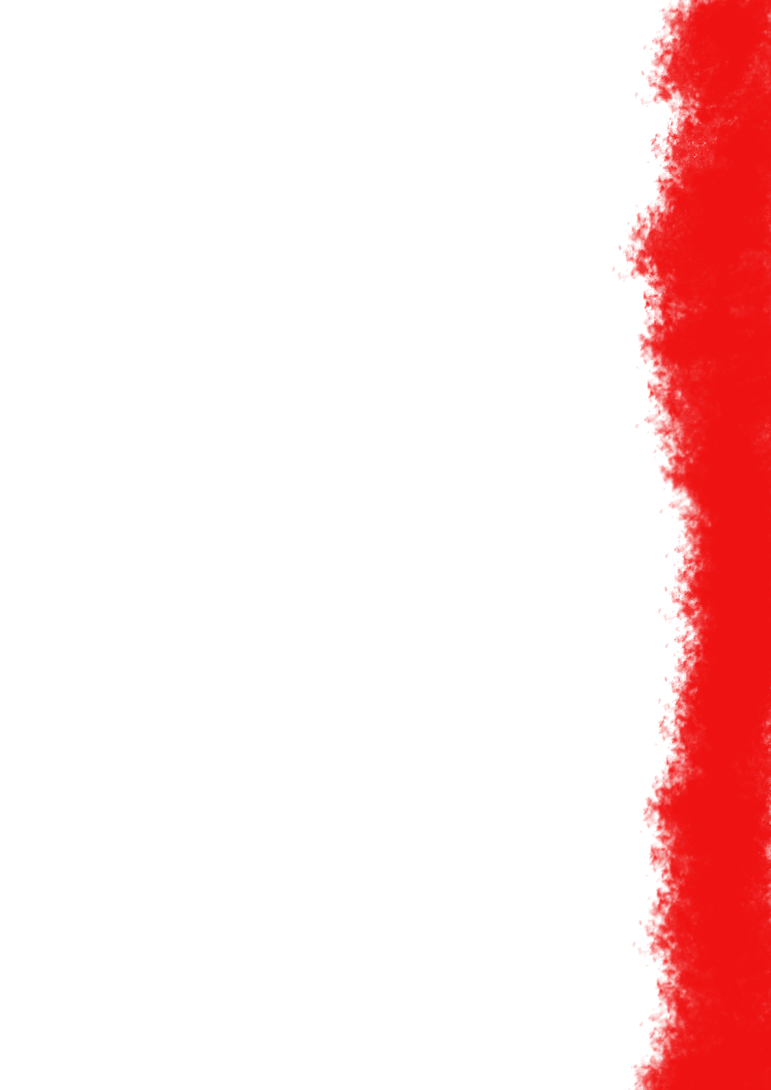
\includegraphics[scale=3.3]{watermarks/test-a.png}}	% página específica
%\newwatermark[oddpages]{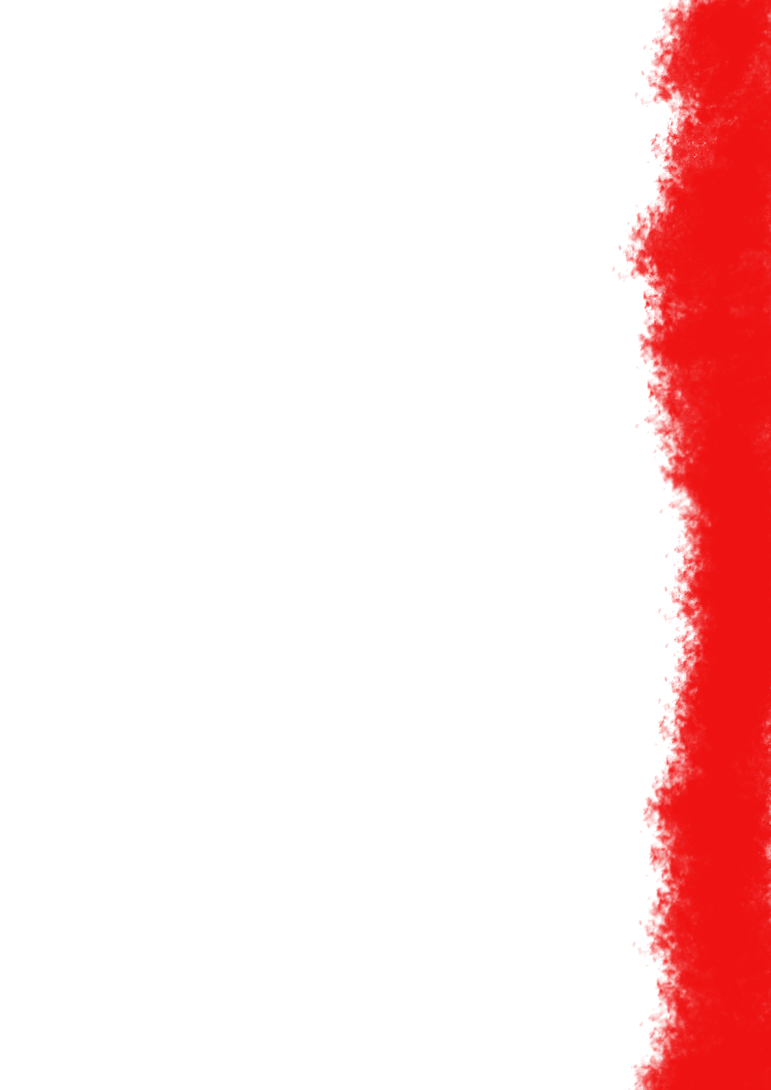
\includegraphics{watermarks/test-a.png}}			% páginas ímpars
%\newwatermark[evenpages]{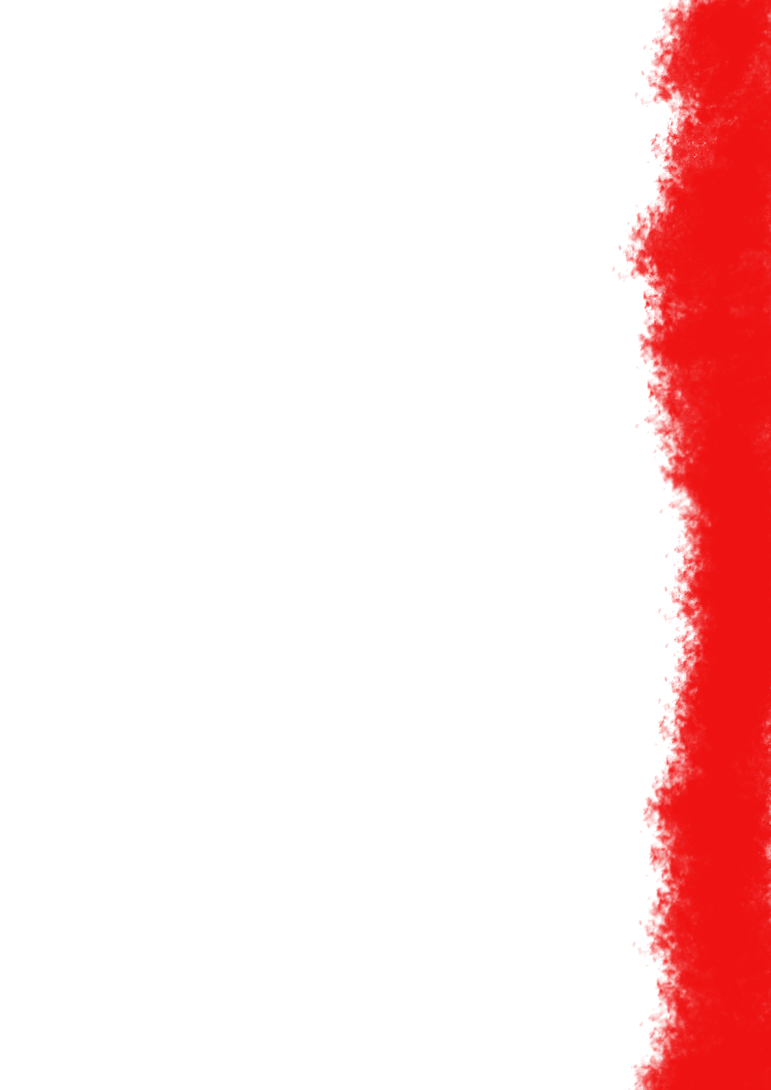
\includegraphics{watermarks/test-a.png}}			% págimas pares
\newwatermark[allpages]{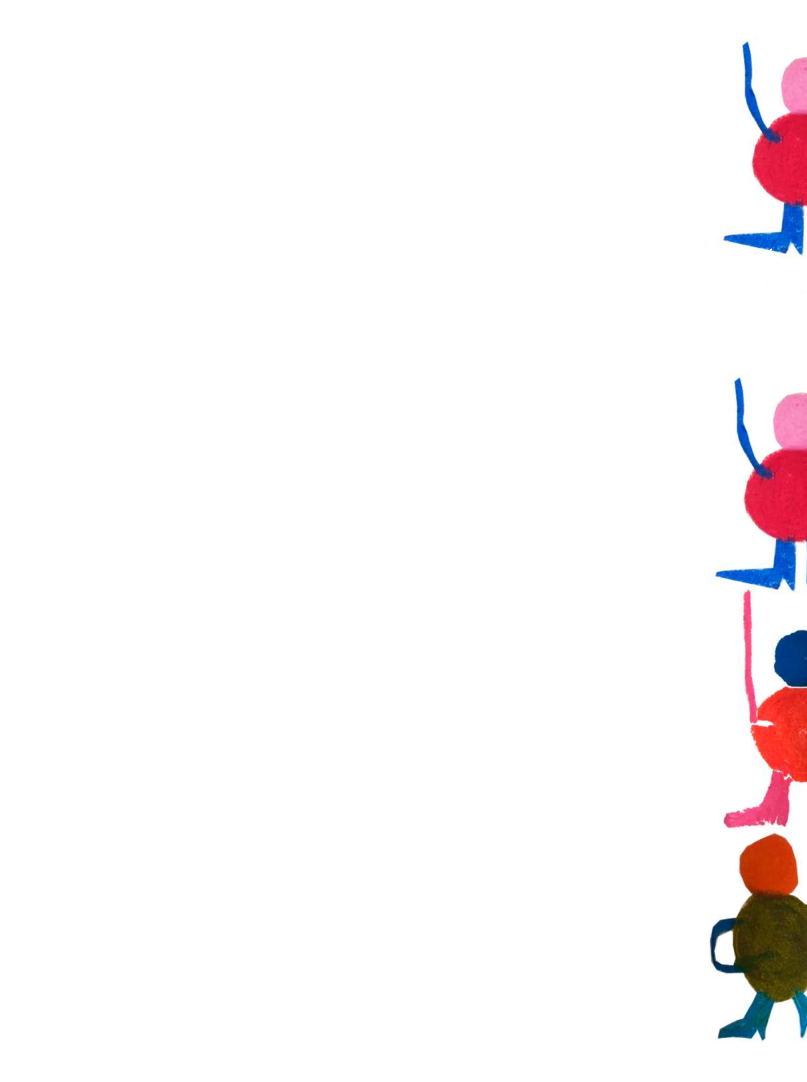
\includegraphics[scale=1]{watermarks/001.png}}

%\pagecolor{cyan!0!magenta!10!yellow!28!black!28!}

\newcommand{\AutorLivro}{Camila Werner}
\newcommand{\TituloLivro}{Bolotas e quadrados}
\newcommand{\Tema}{Relacionamento pessoal e desenvolvimento de sentimentos de crianças nas escolas; nas famílias e nas comunidades (urbanas e rurais)}
\newcommand{\Genero}{Narrativos: fábulas originais; da literatura universal e da tradição popular; etc}
\newcommand{\imagemCapa}{./images/PNLD2022-001-01.jpeg}
\newcommand{\issnppub}{978-65-99441-24-0}
\newcommand{\issnepub}{978-65-99441-27-1}
% \newcommand{\fichacatalografica}{PNLD0001-00.png}
\newcommand{\colaborador}{Paulo Pompermaier e Renier Silva}

\begin{document}

\title{\TituloLivro}
\author{\AutorLivro}
\def\authornotes{\colaborador}

\date{}
\maketitle

%\begin{abstract}\addcontentsline{toc}{section}{Carta ao professor}
%\pagebreak

\tableofcontents



\section{Sobre o livro}

%550 caracteres
\paragraph{O livro} \textit{Bolotas e quadrados}, de Camila Werner, utiliza cores e formas para falar sobre as diferenças da sociedade. Em um mundo habitado por bolotas e quadrados de todas as cores e jeitos diferentes, cada um vai descobrir que, justamente nas diferenças, encontram-se as semelhanças. Assim, todos unem-se para brincar e estar juntos. No jogo entre semelhanças e diferenças, o livro traça aspectos fundamentais ao convívio social e à apreensão do que é conviver com a diferença. É interessante porque toda a narrativa é construída em torno de figuras geométricas coloridas, apresentando, de forma lúdica, as cores e formas para as crianças. 


%822 caracteres
\paragraph{Descrição} Pode-se pensar \textit{Bolotas e quadrados} como um livro em três momentos. No primeiro, aparece o mundo das bolotas. Apesar de todos serem parecidos, pois têm a forma redonda, cada um guarda características peculiares: a cor de sua barriga ou de sua cabeça, o comprimento dos braços, a cor dos pés. No segundo momento, é apresentado o mundo dos quadrados. Igualmente, cada um guarda traços distintivos: as diferentes cores de suas barrigas quadradas, uns que são mais altos, outros mais baixos etc.
No terceiro momento, bolotas e quadrados se encontram. Ao primeiro contato, eles não querem se misturar, pois acham esquisitos aqueles que têm formas diferentes das suas. Logo depois, no entanto, percebem que não há razão para tal separação, e todos se misturam para brincar e se divertir juntos. O livro é disposto de forma que, em uma dupla de páginas, a narração fica ao lado direito, enquanto o esquerdo é ocupado por uma ilustração que representa aquilo que foi narrado, evidenciando as semelhanças e diferenças descritas na história.

%411 caracteres
\paragraph{Competências}
O livro \textit{Bolotas e quadrados} permite trabalhar e explorar diversas competências com as crianças. O próprio enredo da história traz um ensinamento valioso para os pequenos sobre a importância de reconhecer e aceitar as diferenças. Como as diferenças são compreendias em termos de cores e formas, também possibilita o desenvolvimento da apreensão das diferentes cores e formas nas crianças, permitindo ao professor relacionar a narrativa a diferentes objetos do cotidiano, ressaltando suas características no que tange à forma, cor, consistência etc.




%862 caracteres
\paragraph{Aprofundamento} Este material tem a 
intenção de contribuir para que você consiga desenvolver um trabalho aprofundado 
com esta obra na sala de aula. Você encontrará informações sobre a autora, sobre 
o gênero e sobre os temas trabalhados ao longo do livro. Apresentaremos também 
algumas propostas de trabalho para a sala de aula que você poderá explorar livremente, 
da forma que considerar mais apropriada para os seus estudantes. Para a prática 
da Literacia Familiar, oferecemos um guia que pode ajudar nas orientações aos 
responsáveis pela criança, para incentivar o gosto pela leitura e contribuir para 
que os estudantes desenvolvam em casa habilidades que serão importantes no momento 
da alfabetização. Por fim, você encontrará sugestões de livros, artigos e sites 
selecionados para enriquecer a sua experiência de leitura e, 
consequentemente, a de seus estudantes.

\reversemarginpar
\marginparwidth=5cm

\marginnote{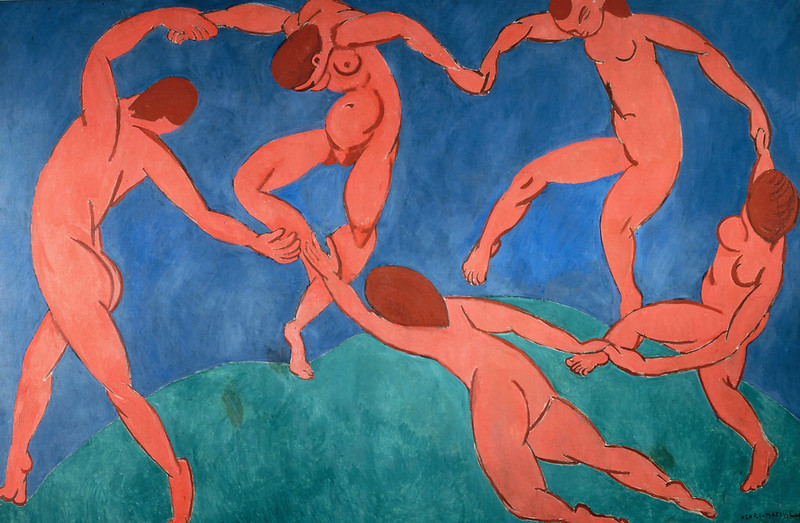
\includegraphics[width=\marginparwidth]{./images/PNLD2022-001-02.png}\\
A autora Camila Werner (Arquivo pessoal)}


\section{Sobre os autores}


%532 caracteres
\paragraph{A autora}
Atua há 18 anos no 
mercado editorial brasileiro e internacional, com experiência 
em diversos segmentos como didático, literatura, trade, 
referência, acadêmico e infantojuvenil, entre outros. 


%313 caracteres
\paragraph{Publicações}
Publicou pela editora Hedra os seguintes livros: \emph{Bolotas e quadrados},
\emph{Esconde-esconde}, \emph{Bom dia, Calu}, \emph{Na casa de Calu}, \emph{Calu e os animais} e
\emph{Calu e as frutas}, todos voltados para o público infantil.


%358 caracteres
\paragraph{Currículo} 
Formada em Comunicação Social com 
especialização em Produção Editorial pela \textsc{eca/usp} 
e mestrado em Books and Digital Media Studies pela 
Universidade de Leiden, Países Baixos.
Atualmente coordena o departamento digital da Brinque 
Book, editora especializada em livros infantojuvenis.


\paragraph{A ilustradora}
Manuella Silveira nasceu em 1999 em São Paulo. Cursa Artes Visuais no Instituto de Artes da Unesp. A pintura vem sendo a prática mais recorrente da jovem artista, e envolve a exploração de um universo pictórico construído a partir de manchas e imagens --- às vezes idiossincráticas, em outras contemplativas --- carregadas de tinta. São temas recorrentes: situações oníricas, personagens irônicos que evocam a tragicomicidade do ser humano e questões de sua infância.


%313 caracteres
\paragraph{Publicações}
Além de \textit{Bolotas e quadrados}, ilustrou os livros \emph{Bom dia, Calu} e \emph{Na casa de Calu}, voltados para o público infantil. Produziu, além de obras literárias, a série de esculturas \textit{Escrachadinhos}, a série de quadros \textit{Onçudinhas}, montou a instalação \textit{Disformidade} e tem outros trabalhos em tela e escultura.


\marginnote{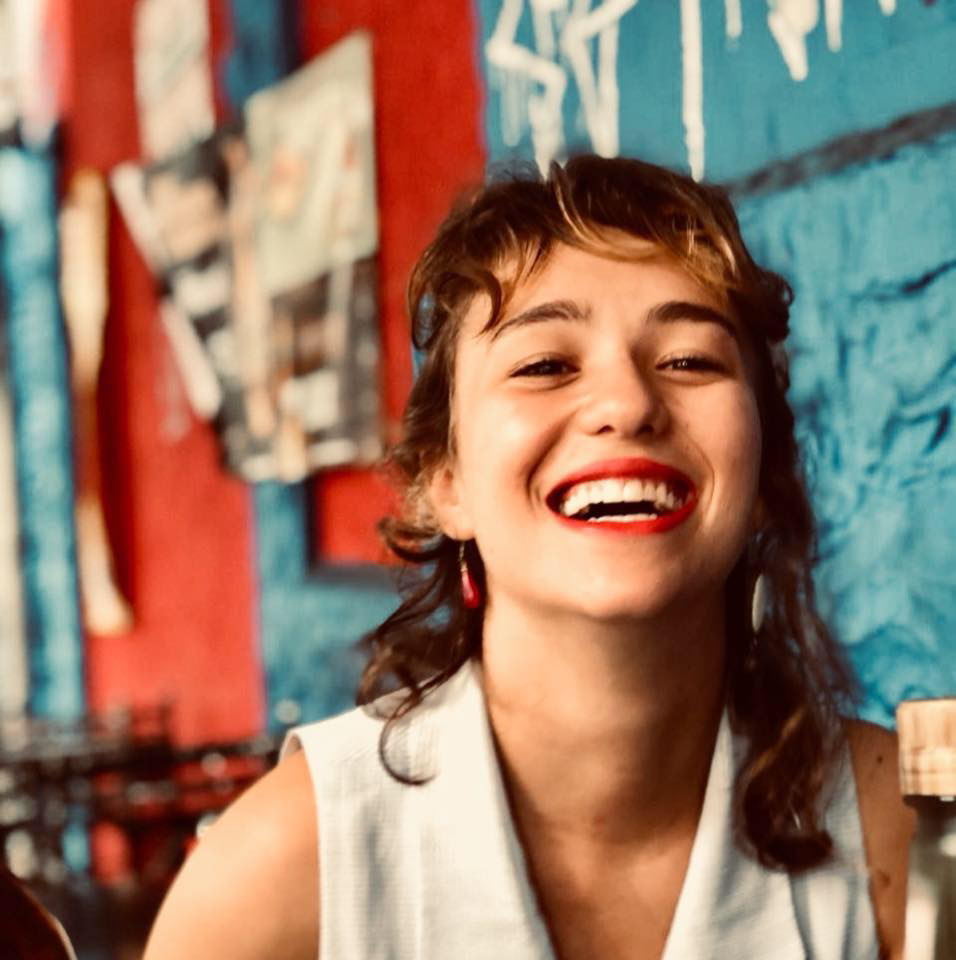
\includegraphics[width=\marginparwidth]{./images/PNLD2022-001-03.png}\\
A ilustradora Manuella Silveira (Arquivo pessoal)}

%358 caracteres
\paragraph{Currículo} 
Em 2018, Manuella Silveira participou da residência de pintura do Festival de Artes da Serrinha, sob orientação do artista Dudi Maia Rosa (que acompanha sua produção em pintura atualmente) e do crítico de arte Rafael Vogt Maia Rosa. Em 2019, foi curadora e produtora da exposição \textit{Grandes Coisas}, do artista plástico Waldomiro Mugrelise, e da exposição \textit{Diga-me Algo Valioso}, do artista argentino Federico Lamas, ambas realizadas no espaço independente Casa Plana.


\section{Sobre o gênero}

%55 caracteres
\paragraph{O gênero} O gênero deste livro é \textit{narrativa}. 


%596 caracteres
\paragraph{Descrição} Em sua base, pode-se definir a narrativa como um gênero que conta uma história, normalmente em estrutura linear, ou seja, começo, meio e fim, e com personagens. 
Dentre os tipos de narrativas mais comuns na literatura infantil, estão: mito, lenda, 
fábula e apólogo. Nos livros infantis, as possibilidades narrativas são quase ilimitadas, pois quase tudo pode integrar a narrativa e fazer parte dela como personagem, já que a capacidade reflexiva das crianças nesta idade ainda está em um nível primário. 

\Image{O gênero da narrativa proporciona ao leitor uma abertura ao mundo. (Pixabay/Tumisu; CC-BY-2.0)}{PNLD2022-001-07.png}

%603 caracteres
\paragraph{Interação} As narrativas são uma forma de inserir os sujeitos no mundo. 
São elas que apresentam boa parte dos valores culturais da sociedade 
onde se vive. Mas não é só passivo o papel das crianças nesta experiência. 
As interações entre dois ou mais personagens onde se verifica
uma ação de linguagem organiza e impulsiona experiências compartilhadas,
importantes para o desenvolvimento psíquico do sujeito nos primeiros anos de vida.
Neste sentido, as narrativas são uma ótima ferramenta para
apresentar o mundo e capacitar as crianças para viver nele, mas como se
trata de um trabalho com a linguagem, sempre dando espaço à individualidade, 
seja na compreensão das histórias, na identificação com as personagens, ou 
no ato de narrar.

%862 caracteres
\paragraph{Competências} 
Através de elementos dos mitos, contos e histórias do cotidiano, desenvolve-se a sensibilidade narrativa e a capacidade de imaginação das crianças. Para um bom desenvolvimento da capacidade narrativa e imaginativa é necessária a intermediação do educador, que vai trazer novos olhares, análises e discussões para ajudar a criança na construção do significado. Essas são etapas fundamentais para o desenvolvimento linguístico e a aquisição das competências de leitura e escrita. Por meio da narrativa, inclusive, a criança passa do diálogo ao monólogo, pois passa a ser capaz de elaborar um discurso para si com maior autonomia, sem a intermediação necessária no diálogo.
O conjunto de elementos verbais e visuais da narrativa proporcionam, assim,
uma abertura ao mundo e um convite para integrá-lo pela curiosidade e pela imaginação.


\section{Temas}

\subsection{Relacionamento pessoal e desenvolvimento de sentimentos de crianças nas escolas; nas famílias e nas comunidades (urbanas e rurais)}

%136 caracteres
\paragraph{Abordagem} O livro relaciona-se ao desenvolvimento das relações pessoais e dos sentimentos coletivos, uma vez que aborda o contato entre dois grupos de personagens diferentes que, após um conflito inicial, aprendem a aceitar as diferenças para viver em harmonia.

%206 caracteres
\paragraph{Descrição} O livro oferece uma ótima oportunidade de explorar 
e aprofundar os sentimentos de respeito à diferença, contribuindo para uma melhor compreensão das diferentes configurações sociais e, inclusive, desenvolvendo o respeito e a atenção ao próprio corpo.

%275 caracteres
\paragraph{Competências} Este tema relaciona-se, principalmente, ao 
campo da experiência O eu, o outro e o nós 
descrito pela \textsc{bncc}, que explora as relações interpessoais das crianças e sua capacidade de criar vínculos, percebendo as diferenças que constituem a sociedade e aprendendo a respeitá-las.


\section{Modelagem de aula}
A seguir você encontrará a descrição de uma aula modelo como exemplo 
prático de exploração do livro com estudantes. Esta seção apresentará 
orientações sobre como organizar a sala de aula para receber os 
estudantes, exercitar a interação verbal e prepará-los para o 
momento da leitura.

Em seguida, você encontrará a \textbf{Leitura dialogada}, um 
tópico destinado a te orientar para o momento específico da 
leitura com os estudantes. Por fim, no tópico 
\textbf{Propostas de atividades}, você encontrará ideias 
de práticas que pode explorar com as crianças em sala de 
aula antes, após e durante a leitura. 

Essas atividades podem ser trabalhadas de acordo com a 
disponibilidade do seu cronograma. Fique à vontade para adaptá-las 
da forma que achar melhor para os seus estudantes. Cada turma é única 
e o seu conhecimento prático das características de cada aluno será 
essencial para definir a melhor forma de aplicar essas ideias. 

O objetivo deste manual é oferecer algumas ideias 
e inspirações para um trabalho que pode ser desenvolvido tanto 
a curto, quanto a médio e longo prazo. Sinta-se à vontade para 
personalizar a aula e torná-la sua, aplicando seus conhecimentos, sua 
personalidade e aproveite para fortalecer 
seu vínculo com a turma.


\subsection{Antes de ler}

\BNCC{EI02EO02}
\BNCC{EI02EO03}
\BNCC{EI02EO04}
\BNCC{EI02EO06}
\BNCC{EI02ET01}
\BNCC{EI02ET04}
\BNCC{EI02CG02}

%Alterar o nível escolar nesse parágrafo.
Como este trabalho será realizado com crianças da \textbf{Creche 2}, 
que ainda não têm tanta intimidade com o livro enquanto objeto, você terá o 
papel essencial de mediar este contato. 

Nosso objetivo é que os próprios estudantes possam manusear 
e explorar o livro de forma autônoma, mas, para que isto aconteça, você 
pode ajudar a tornar o caminho mais convidativo com atividades que tenham 
intencionalidade educativa. 

A \textsc{bncc} define intencionalidade educativa como ``organização 
e proposição, pelo educador, de experiências que permitam às crianças 
conhecer a si e ao outro e de conhecer e compreender as relações com a 
natureza, com a cultura e com a produção científica, que se traduzem nas 
práticas de cuidados pessoais (alimentar-se, vestir-se, higienizar-se), 
nas brincadeiras, nas experimentações com materiais 
variados, na aproximação com a literatura e no encontro com as 
pessoas''.\footnote{\textsc{bncc}, página 39}

É importante manter essa intencionalidade em mente não apenas na condução 
das atividades propostas neste manual, mas também para aproveitar as 
oportunidades espontâneas de construir conhecimentos que podem surgir durante 
a interação direta com os estudantes.

\begin{enumerate}
%836 caracteres
\item \textbf{O ambiente}\quad Antes de iniciar o trabalho com o livro, é importante que você 
prepare o ambiente para receber a turma. Como o trabalho com o livro terá 
três momentos (antes, durante e depois da leitura), seria interessante que você 
criasse um ambiente para cada etapa. Nas \textbf{Sugestões de referências complementares} 
você encontrará um artigo que discorre sobre a importância da organização da sala 
de aula para a educação infantil, que pode ser um bom guia para a criação desses 
ambientes.
Para o momento antes da leitura, sugerimos uma atividade que objetiva estimular o trabalho corporal e sensorial, a motricidade, os conceitos de perto, longe, dentro, fora e o controle de força e impulso. Dessa forma, contribui para desenvolver a lateralidade e o controle emocional. Se for realizada em sala de aula, o professor precisará afastar as cadeiras e mesas para ter um espaço aberto. 

%413 caracteres
\item \textbf{Materiais}\quad Algo em torno de 5 ou 6 caixas médias de papelão, 5 ou 6 bolas médias, que podem ser produzidas pelos alunos com papel ou retalhos.

%632 caracteres
\item \textbf{Desenvolvimento}\quad O educador deverá organizar as caixas uma ao lado da outra, em uma distância que não atrapalhe o arremesso da bola. Primeiro, o professor deve mostrar aos alunos os materiais e dizer que a bola é um círculo e a caixa um quadrado, questionando-os se percebem essa diferença. Após o diálogo, explique a atividade e divida  os alunos em grupos para realizar os arremessos. Cada grupo terá sua própria caixa e bolas para arremessar. A distância para o arremesso deve ser pensada de acordo com a faixa etária e habilidades do aluno. Forme filas por ordem alfabética, realize o arremesso para mostrar como se faz e treine com todos. Quando todos entenderem a atividade, inicie pelo primeiro da fila de cada grupo e assim por diante. Cada aluno terá direito a 3 arremessos por vez. Durante os arremessos, ensine conceitos como dentro/fora, longe/perto. Auxilie-os a acertar, mostrando como se faz. Estimule que os maiores ajudem os menores. 

\item \textbf{Perguntas para avaliar}\quad As crianças respeitaram as regras do jogo? Como resolveram os conflitos? Como se comportaram quando não conseguiam acertar o proposto? Elas buscaram diferentes estratégias do que foi explicado? 

\end{enumerate}


\subsubsection{A interação verbal} 
Criar situações em que as crianças precisam dialogar diretamente com 
você é uma das práticas mais importantes de Literacia, pois elas estimulam 
o desenvolvimento linguístico, ampliam o vocabulário e reforçam a 
capacidade dos estudantes de compreenderem o que ouvem e se expressarem 
pela fala. O diálogo livre com a criança também reforça sua autoestima, pois 
a faz se sentir ouvida e valorizada pelo adulto, ao vê-lo prestar atenção 
no que ela tem a dizer. Portanto, sempre que possível, reserve um tempo na 
aula apenas para a interação verbal. 

\Image{A atenção às formas de expressão é imprescindível para uma comunicação de qualidade. (Ministério do Desenvolvimento Social; CC-BY-SA-2.0)}{PNLD2022-001-10.png}

Como esse tipo de interação é espontânea e intimamente atrelada ao 
desenvolvimento de cada estudante, nossas orientações não serão específicas. 
A ideia é que você adapte este momento de acordo com as respostas e os 
repertórios das crianças. É um momento de estreitamento de vínculos e, portanto, 
fique à vontade para ser espontânea e para explorar os tópicos que achar 
mais interessantes para a sua turma.

Inicie as conversas com naturalidade, seguindo os objetos de atenção das crianças. 
Você pode partir de objetos que estejam analisando
para iniciar um assunto e incentivar que se expressem. Ainda que a
criança não fale corretamente, continue interagindo, 
pois a intenção aqui é que a criança perceba que outras pessoas estão respondendo 
à sua comunicação. 

Fique atento a todas as formas de expressão: os gestos, as falas, as 
expressões faciais, para onde olham\ldots{} tudo pode ser explorado durante a conversa. 
Demonstre curiosidade sobre eles, seja um ouvinte entusiasmado e incentive que eles 
conversem entre si. Faça perguntas e construa a resposta junto com as crianças. 

A seguir, algumas dicas que podem contribuir para que a interação verbal 
seja produtiva em sua sala de aula: 

\begin{enumerate}
\item Sente-se no chão e brinque com eles, estabelecendo 
contato visual. Além das pequenas frases que conseguem formar, vocalizações, 
gestos e expressões faciais podem ser boas formas de comunicar.

\item Não se esqueça que a conversa é uma troca e, portanto, 
evite ficar falando sozinho ou desvalorizar as respostas das 
crianças quando não conseguem formular frases completamente articuladas. 
Nunca descarte uma tentativa de comunicação. 

\item Evite utilizar falas negativas que desencorajam o diálogo. 
Se precisar que a turma 
corrija algum comportamento, explique claramente a razão e 
oriente com calma. Incentive positivamente as crianças e 
destaque o motivo de seus elogios. 

\item Aproveite alguns momentos durante a conversa para chamar 
a atenção das crianças para os sons das palavras e das letras que você 
acabou de usar ou que eles pronunciaram.  

\item Explore possibilidades de interação como apontar e 
nomear objetos, pessoas e animais, imitar a criança ou pedir que 
ela o imite, fazer caretas, reproduzir sons de 
animais para que repitam, ensinar os nomes de partes do corpo, 
entre outras atitudes que estimulem a comunicação com a criança. 

\item Muitas dessas dicas poderão ser aproveitadas pela 
família durante a prática da Literacia Familiar. Portanto, 
se achar necessário, compartilhe algumas destas orientações 
com as famílias dos estudantes.
\end{enumerate}


\subsection{A leitura dialogada}
Este é o momento em que será realizada a leitura propriamente dita. 
Se possível, crie um \textit{cantinho da leitura} em sua sala de aula. Um 
ambiente confortável, de preferência em que todos se sentem no chão ou 
em pufes para que consigam enxergar as ilustrações do livro que está 
sendo lido e interagir com facilidade. Se houver possibilidade, mantenha 
sempre os livros da turma em uma altura da estante que permita fácil 
acesso para os estudantes ou guarde os livros em uma caixa que as crianças 
possam mexer com autonomia. É importante que elas tenham autonomia para 
acessar os livros e se sintam à vontade para pegá-los sempre que quiserem. 

\Image{É importante que o cantinho da leitura proporcione autonomia para as crianças. (Fotos Públicas/Marina Cajaíba; CC BY-NC 2.0)}{PNLD2022-001-08.png}

Outra possibilidade de ambiente para esta leitura, se a escola permitir, 
é efetuar essa leitura ao ar livre, embaixo de uma árvore, onde as crianças 
possam ouvir os sons dos pássaros e sentir o cheiro da grama. Sair da sala 
de aula pode oferecer um ótimo leque de experiências aos seus estudantes e 
reforçar a conexão entre os estudantes em diferentes ambientes.  

Reserve uma boa parte da aula para o momento da leitura com os estudantes, 
pois é importante que esse momento aconteça sem pressa. O objetivo da 
leitura dialogada é que seja uma leitura em bate-papo. A criança deve 
assumir um papel ativo na leitura, mesmo que ainda não seja capaz de 
ler sozinha. Além de promover o gosto pela leitura, esta prática estimula 
o desenvolvimento da linguagem, enriquece o vocabulário e 
aumenta o conhecimento de mundo.

%Especificar o livro.
No caso de \textit{Bolotas e quadrados} o diálogo durante a leitura é 
ainda mais importante, considerando que as crianças ainda não têm domínio sobre o código escrito e, portanto, a compreensão do texto se apoiará principalmente na sua interação com elas. 
Você deve interagir com eles durante toda a 
leitura, fazendo perguntas e partindo de detalhes do livro para 
levantar novas questões. 

A seguir, algumas orientações para aproveitar este momento e desenvolver uma atividade durante a leitura: 

\begin{enumerate}
%177 caracteres
\item \textbf{Contexto}\quad Após a atividade anterior à leitura, conceitos mobilizados pelo livro, como as diferentes formas, ainda estarão frescas nas crianças, que brincaram e se divertiram usado apenas bolotas e quadrados. A partir do livro, propõe-se uma leitura que  
proporcione um momento no qual os alunos possam se movimentar e participar ativamente do contexto e da leitura. Prepare o material antecipadamente para que, durante a leitura, os alunos possam associar os materiais concretos às imagens do livro.
Assim, poder-se-á trabalhar a linguagem, a oralidade, as diferenças e as formas de maneira a relacionar a leitura e objetos concretos. 
Aconselha-se o professor a se sentar em roda com as crianças, em sala de aula, biblioteca ou espaço externo.

\item \textbf{Materiais}\quad Livro \textit{Bolotas e quadrados}; formas geométricas de quadrados, círculos e triângulos grandes cortados em papelão e revestidas com \textsc{eva} colorido.


\item \textbf{Desenvolvimento}\quad Distribua o material de acordo com o número de crianças em sala, atentando-se para que todos tenham ao menos uma forma geométrica colorida em mãos. Reúna os alunos e sentem-se em círculo, para que todos possam participar. Antes de iniciar a leitura entregue para cada um círculos, quadrados ou triângulos. Promova o diálogo entre os alunos acerca das formas e cores. Ao iniciar a narração, possibilite que as crianças comparem os brinquedos às imagens do livro.
 
%230 caracteres
\item \textbf{Manuseio}\quad Deixe que as crianças manuseiem o livro 
e explore com elas todos os elementos que o compõem. Mostre o que é a 
capa e onde estão as páginas. Deixe que coloquem as figuras que têm em mãos sobrepostas às ilustrações do livro, vendo se conseguem identificar corretamente os quadros e círculos e associar as figuras do livro aos materiais que manuseiam.

%495 caracteres
\item \textbf{Diálogo}\quad Como as personagens do livro são bolotas e quadrados, as crianças terão oportunidade de tê-las em mãos e sentir que as protagonistas da história saíram do livro para brincar com elas. Use frases como: ``João está com o quadrado vermelho, Ângela com o círculo amarelo, olhem o círculo e o quadrado na história, parece que as formas saíram do livro para brincar com vocês''. Incentive o diálogo entre as crianças, que podem comparar as suas figuras e estabelecer relações com a narrativa, pois cada bolota e quadrado é diferente e, mesmo assim, todas podem brincar juntos.

%346 caracteres
\item \textbf{Escuta}\quad Elogie atitudes positivas, como 
a boa interação com a história lida e a solicitação de interagirem com ela. Se os estudantes tentarem 
tomar o seu lugar e começar a falar sobre a história ou as figuras que têm em mãos, valorize e escute com atenção o que estiverem falando. Mas não 
force a leitura. Se as crianças estiverem cansadas, faça outra atividade 
e retorne depois. 

\includepdf[nup=2x3, 				% grid
			%offset=-15mm -5mm, 	% posição
			scale=.8, 				% tamanho da página
            delta=4mm 4mm, 			
            frame,
            pages={10-15}]{./pdfs/\jobname_MIOLO.pdf}

%935 caracteres
\item \textbf{Leitura}\quad Enquanto lê, sugere-se que a professora mostre as figuras para as crianças e estimule que elas discutam sobre o que está sendo mostrado.
Mostre como são diferentes e parecidas, estimule a troca de informações sobre os materiais entre as crianças. Promova um ambiente livre e imaginativo no momento de leitura. 
Faça perguntas como:

\begin{itemize}
\item Qual a diferença entre essas duas bolotas?
\item Qual tem o pé azul?
\item Qual tem o braço mais comprido?
\end{itemize}

Se as crianças não souberem responder, aponte no livro as figuras que correspondem às questões colocadas. Estabeleça relações entre as perguntas e as figuras que as crianças estão manuseando, com indagações como:

\begin{itemize}
\item Essa bolota é maior que a outra. Quem tem a bolota maior?
\item Quem tem bolotas e quem tem quadrados?
\item Qual é o quadrado azul?
\item E o triângulo, alguém sabe onde ele está?
\end{itemize}

Dessa forma, estimula-se a apreensão das diferenças entre cores e formas de maneira dinâmica e lúdica, aumentando a interação com o momento da leitura. Assim, o hábito da leitura passa a estar associado a momentos dinâmicos e divertidos.
Como no livro, apesar das diferenças, todos brincam juntos, é interessante sugerir essa dinâmica na sala também: pode-se pedir, por exemplo, que os alunos componham novas figuras juntando diferentes quadrados e círculos. Ou pedir que formem grupos diversificados, em que é preciso ter um número parecido de crianças com bolotas e quadrados. 


%382 caracteres
\item \textbf{Interação}\quad Nomeie as ilustrações 
do livro, apontando para elas com o dedo e, ao mesmo tempo, reforçando sua ligação com a palavra que a representa. Por exemplo, quando a narrativa fala de ``gente que é mais baixa'', aponte as figuras mais baixas, realçando a diferença de tamanho entre as figuras.
Destaque os sons de algumas 
palavras mais difíceis. Interrompa a leitura em alguns momentos e peça que 
os estudantes repitam palavras e sentenças do livro. Se possível, 
releia a mesma história outras vezes ou recrie narrativas em cima do livro, perguntando aos estudantes, por exemplo, do que mais as bolotas e quadrados poderiam brincar juntos, ou quais outros mundos podem existir habitados por outras formas geométricas.

\item \textbf{Perguntas para avaliar}\quad Os alunos gostaram da atividade? Usaram a criatividade? Conseguiram identificar semelhanças e diferenças entre as formas e as imagens do livro?  Como se comportaram durante a leitura? 
\end{enumerate}


\subsection{Propostas de atividades}

\BNCC{EI02CG01}
\BNCC{EI02CG02}
\BNCC{EI02CG03}
\BNCC{EI02CG05}
\BNCC{EI02ET01}
\BNCC{EI02EF03}
\BNCC{EI02EF04}


\begin{enumerate}
%700 caracteres
\item \textbf{Contexto}\quad A proposta trabalhará o fortalecimento da identidade dos alunos, a capacidade de reconhecimento do eu e do outro e a habilidade de realizar movimentos coordenados em grupo. A participação dos pais será necessária, por isso deverão ser comunicados antecipadamente. 

\Image{Nessa atividade, é importante incentivar as crianças a cantarem junto. (Secom/Bruno Rocha; CC BY-NC 2.0)}{PNLD2022-001-09.png}

\item \textbf{Materiais}\quad Caixa de som ou aparelho de vídeo; camisetas coloridas para as crianças. 

%650 caracteres
\item \textbf{O ambiente}\quad Sala de aula, espaço externo ou sala de vídeo. 

%950 caracteres
\item \textbf{A atividade}\quad Com um tempo adequado para os pais se organizarem, estipule uma data para o dia da atividade. Peça para os responsáveis auxiliarem as crianças na escolha de uma camiseta colorida para o dia da aula. Oriente-os sobre a importância de deixar a criança escolher sozinha, pois sua função é apenas facilitar o processo de escolha. Antes de conversar com os pais, promova um diálogo em que os pequenos possam contar qual sua cor preferida em sala de aula. Mostre cores para os menores, que ainda não desenvolveram a linguagem mais complexa. Estimule que escolham, mas não tenha uma postura rígida quanto a isso, o importante é a escolha em casa. No dia da atividade, peça para as crianças contarem como foi a escolha e ajude-as a vestir a roupa escolhida.

Reúna as crianças em roda e coloque para tocar a música  ``Magia das cores'', do Mundo Bita.\footnote{Disponível em: \url{https://www.youtube.com/watch?v=EW1Is3BVp5U}.} Dancem em roda de mãos dadas, entusiasme as crianças a tentarem cantar. Após o momento musical, reunidos em roda e de mãos dadas, inicie a atividade de roda das cores. Observe as cores das camisetas das crianças e estimule a interação entre a associação e identificação das cores e movimentos corporais.
Por exemplo:

 
\begin{itemize}
\item Maria está de vermelho, quem está de vermelho dê um passo à frente;
\item Agora, que está de azul dê um passo para trás;
\item Quem está de branco troque de lugar com quem está de rosa;
\item Quem está de vermelho, volte um passo atrás.
\end{itemize}

Repita a brincadeira até que tenha dito o nome e a cor de todas as crianças. Auxilie as crianças menores. Use como inspiração as diferenças e dinâmicas abordadas pela narrativa do livro.

%550 caracteres
\item \textbf{Interação}\quad A estrutura da atividade é toda baseada na interação entre as crianças, o professor e a história do livro. Após a dinâmica, o professor pode retornar ao livro para que as crianças o manuseiem. Observe o comportamento dos alunos, se eles mudaram de opiniões após as brincadeiras ou se apresentam outra percepção sobre as diferenças e características das personagens. Pode-se, por exemplo, perguntar o que mais elas apresentam de diferente além do enunciado na narração.
 Incentive que eles tentem repetir algum trecho da história e
faça perguntas que os estimule. Como as crianças vão estar com roupas coloridas, pode-se fazer as mesmas perguntas do enredo para elas: ``Há pessoas que vestem azul e outras que vestem vermelho''; ``Quem está de vermelho? E de azul?''; ``Entre os de vermelho, quem tem o braço mais comprido?''; ``Quem tem calçados coloridos?'' etc.
Quando as crianças propuserem suas ideias, interaja com o pensado e apresentado pelas crianças, fazendo perguntas que as auxiliem a desenvolver o pensamento iniciado.

\item \textbf{Perguntas para avaliar}\quad Os alunos conseguiram escolher? E os menores?  Como foi o relato dos pais sobre o processo de escolha? As crianças dançaram? Cantaram? Se divertiram? Conseguiram fazer o propósito de ir para frente e para trás? 
\end{enumerate}


\section{Literacia familiar}
O \textsc{pna} dá destaque especial para a importância do envolvimento da família 
no processo pedagógico nesta faixa etária e denomina Literacia Familiar o conjunto 
de experiências e práticas relacionadas à linguagem (oral, escrita ou lida) vivenciadas 
com os cuidadores. 

Essas estratégias podem começar a ser colocadas em prática desde a 
gestação e continuar até o final da adolescência. São práticas simples e divertidas 
que estimulam o desenvolvimento de quatro atividades fundamentais: ouvir, falar, 
ler e escrever que criam momentos de afeto e interação para a família. 

Para que esse trabalho conjunto entre escola e família funcione, é 
fundamental que a escola esteja em constante diálogo com os responsáveis e 
você consiga orientá-los. Um grupo em aplicativos de mensagens instantâneas ou um 
grupo de e-mails são saídas viáveis para que a comunicação se estabeleça e pode ser 
uma forma útil das famílias compartilharem suas vivências e trocarem sugestões 
de abordagens, sempre contando com a sua mediação. 

Com o objetivo de incentivar 
a prática da \textit{literacia familiar}, se possível, organize um rodízio entre os familiares 
das crianças para emprestar o livro da biblioteca da turma. Neste caso, crie um caderno 
de registro e estabeleça períodos para cada família ficar com o livro. É importante 
que os familiares compreendam a seriedade deste compromisso, pois o livro pertence 
ao acervo da sala e, portanto, deve ser bem cuidado e devolvido na data acordada. 

Se não for possível garantir o acesso direto dos cuidadores da criança ao livro, 
grave um vídeo direcionado a eles, contando a história e apresentando algumas 
das ilustrações. O importante é que os familiares saibam com clareza qual livro 
está sendo trabalhado, a história contada e se sinta seguro para explorar as temáticas 
do livro com a criança. Orientações claras e a manutenção do canal de comunicação com 
os responsáveis é essencial para que eles se sintam seguros e à vontade para fazer perguntas 
se tiverem dúvidas. 

Neste manual, você encontrará algumas práticas que podem ser 
recomendadas aos familiares para ajudá-los a expandir e aprofundar o trabalho 
que você iniciou em sala de aula.


\subsection{Importância da leitura}
Na escola, aprendemos a ler letras, mas é importante ter em mente que nós 
lemos o mundo desde muito pequenos: “lemos” os animais que passam pelos nossos 
quintais, a expressão no rosto dos nossos familiares, as cores que pintam o céu 
em um fim de tarde. 

Vamos aprendendo, ao longo da vida, a interpretar acontecimentos 
e sons que escutamos e a utilizá-los para nossa comunicação. Aprender a ler textos e 
escrevê-los expande a nossa leitura do mundo, pois permite que sejamos capazes de 
interpretar um código e experimentar, a partir dele, novas experiências e conhecimentos. 

O simples contato com os livros já permite um leque grande de sensações: 
sentimos as texturas, as formas, vemos as cores do livro, escutamos o som da página 
virando e o som da voz do narrador, se a história estiver sendo lida em voz alta. Para uma 
criança pequena, são experiências que podem contribuir diretamente com o desenvolvimento psicomotor 
e cognitivo. 

Nosso papel, enquanto mediadores de leitura, é contribuir para que essas 
sensações sejam associadas a momentos positivos, de construção de 
conhecimento e exercício de imaginação. 

Com os livros, podemos conhecer mais da história humana, descobrir informações 
novas sobre sociedades diferentes da nossa, imaginar situações e contextos inéditos 
para nós e aumentar o nosso repertório. São por meio deles que melhoramos nossa 
capacidade de interpretação, de expressão, de análise e senso crítico. Boas habilidades 
leitoras podem contribuir para o desenvolvimento de um estudante em todas as outras 
disciplinas, pois exercem influência direta na forma como absorvemos e 
construímos conhecimento.


\subsection{O papel da família na formação do leitor}
A família é peça fundamental na formação do leitor, pois é ela quem primeiro 
ensina a criança a ler. Não apenas os textos escritos, mas a ler o mundo, a 
interpretar os estímulos que a cercam, a construir seu próprio vocabulário e a 
comunicar seus pensamentos e necessidades.

O universo das letras é muito presente na vida das crianças antes mesmo de sua 
entrada na escola. Aparece nas histórias e ilustrações do livro que o cuidador 
lê ao colocá-la para dormir, nas situações em que vê os responsáveis se comunicarem 
pela escrita ou nos textos que podem permear seu cotidiano (nos outdoors, na 
televisão, no celular, manuais de instrução entre outros). 

Os familiares têm, 
portanto, uma ótima oportunidade de apresentar a leitura com leveza, de forma 
prazerosa, associado ao contexto em que a criança vive e à momentos de diversão. 
Você poderá orientar os pais nesta tarefa, ensinando-os com este guia a aproveitar 
as oportunidades para trabalhar a Literacia com a criança.


\subsubsection{Práticas de literacia familiar} 

São muitas as experiências que a prática da \textit{literacia familiar} 
pode oferecer às crianças. A seguir, explicamos cada uma delas para que você possa, 
se achar necessário, compartilhar com os responsáveis enquanto estiver orientando-os: 

\paragraph{Interação verbal} Aumentar a quantidade de conversas com as 
crianças, fazendo perguntas para incentivar o diálogo.

\paragraph{Leitura dialogada} Interagir com a criança durante a leitura 
em voz alta, criar expectativa sobre o livro, chamar a atenção para detalhes 
das ilustrações e comentar o enredo.

\paragraph{Narração de histórias} Interagir com a criança enquanto 
estiver narrando uma história, por exemplo, incluindo-a na ação, utilizando 
marionetes ou permitindo que ela complete a narrativa.

\paragraph{Contatos com a escrita} Apresentar as letras para as 
crianças, incentivar que tentem escrever ou ler, ajudá-los a desenhar letras, 
entre outras formas de incentivar o contato com as palavras.

\paragraph{Atividades diversas} Qualquer atividade com a criança 
pode ser utilizada para contribuir para a alfabetização. Jogos, brincadeiras, 
instrumentos musicais, canto, dança, passeios e viagens oferecem boas 
oportunidades de aprendizado.

\paragraph{Motivação} Atitudes que motivem as crianças à envolver-se com 
o mundo da leitura e da escrita.

\subsection{Exercitando a literacia familiar}

\BNCC{EI02EF01}
\BNCC{EI02EF03}
\BNCC{EI02ET01}
\BNCC{EI02ET05}

\begin{enumerate}
%700 caracteres
\item \textbf{Como começar}\quad O contato da família com a criança e o livro começam desde a primeira atividade proposta.
Dialogue com os pais e mostre como a mesma atividade de pré-leitura (de brincar com objetos de diferentes formatos) pode ser realizada em casa com objetos do cotidiano, como brinquedos pequenos, caixas e potes. Esclareça o objetivo e a importância para o desenvolvimento. 
Peça que os familiares conversem com as crianças a respeito das diferentes características que cada objeto tem, ressaltando aspectos como forma e cor.
As crianças, com ajuda dos pais, podem fazer um desenho que represente essas diferenças entre os objetos e trazer para a sala de aula, socializando com os colegas.
Essa é uma forma de iniciar o contato dos pais com as crianças na leitura, pois os envolve nas atividades e competências que serão desenvolvidas em sala de aula.

%650 caracteres
\item \textbf{Leitura}\quad A família pode continuar 
explorando os temas apresentados pelo livro. Uma das formas de fazer isso é solicitar aos pais introduzam os conceitos de cor e forma no dia a dia do aluno. Através dos objetos de casa, os responsáveis podem incentivar a aquisição desse conhecimento com as crianças.
É interessante fazer comparações entre os objetos, por exemplo: o tapete é quadrado, a janela também; a bolacha é redonda, o ovo também é um círculo; e assim por diante. Esta proposta estimula a generalização do conhecimento aprendido em sala de aula.
Os pais podem relacionar essas semelhanças e diferenças com o livro lido em sala: mostrando as semelhanças entre as personagens e os objetos do cotidiano, que também são encontrados nas mais diversas formas, tamanhos e cores.
Outra possibilidade, quando a família tem acesso ao livro, é ler alguns trechos com a criança em um horário estipulado para isso. A leitura em família é importante pois relaciona o ato de ler e manusear um livro com o campo de suas experiências afetivas.

%1073 caracteres
\item \textbf{Instrução}\quad Informe aos pais sobre a estrutura do livro e as principais competências desenvolvidas em sala de aula.
Oriente-os a, quando possível, ler alguns trechos da história com a criança, confabulando sobre os formatos e cores distintos encontrados em casa.
Incentivando a percepção sobre diferenças e semelhanças no cotidiano da criança, elas começam a perceber as relações de generalização que estruturam o livro.
Desta forma, as crianças vão relacionando as experiências de semelhança e distinção do livro ao seu cotidiano.
Ademais, quando os responsáveis leem com as crianças, colocam-na em contato com duas experiências de leitura distintas: através da mediação em sala de aula e em família. 
Mesmo pequenas, as crianças conseguem perceber a diferença entre 
as formas de contar, e elementos da narração em casa podem ajudá-la a compreender 
sentidos e perceber detalhes que não foram explorados em sala de aula. Se possível, depois da leitura, oriente 
que voltem ao livro e tentem identificar as personagens e as semelhanças e diferenças que as caracterizam.
Os pais também terão papel fundamental em uma das atividades propostas nesse material, a de a criança escolher sua própria roupa para ir à escola. Explique como a atividade fortalece a identidade e a autoestima. Esclareça para os pais como esta simples orientação estimula o desenvolvimento. 

Outra opção é entregar o livro para a criança e pedir que ela tente se lembrar
do que foi falado em sala de aula, quais elementos foram destacados e enfatizados pelo educador e pelos colegas. Pode-se orientar os pais a pedir que a criança conte sobre as atividades realizadas em sala, tentando se lembrar das figuras que foram manuseadas e das diferentes roupas de seus coleguinhas, pois isso estimula a criatividade e a memória dos alunos. Mesmo que a memória não pareça 
completa para o adulto, é importante que ele ouça com atenção e 
valorize todas as tentativas da criança. Afinal, ao tentar recontar, 
ela manipulará o livro, treinará a coordenação motora, conhecerá as texturas 
do objeto e poderá imitar a forma como o adulto 
conta a história, treinando a fala. 
\end{enumerate}

 
\section{Sugestões de referências complementares}

\subsection{Livros} 

\begin{itemize}
\item \textsc{lins}, Guto. \textit{Livro infantil? projeto gráfico, metodologia, subjetividade}. São Paulo: Rosari, 2002.

Livro que aborda a importância das escolhas visuais (ilustração, projeto gráfico, lettering) na literatura infantil.  

\item \textsc{hunt}, Peter. \textit{Crítica, teoria e literatura infantil}. São Paulo: Cosac Naify, 2010.

Livro sobre crítica de literatura infantil que contêm definições de livro ilustrado e livro imagem. 
\end{itemize}

\subsection{Artigos}

\begin{itemize}
\item \textsc{sardelich}, Maria Emilia. Leitura de Imagens, Cultura Visual e Prática Educativa. 
In: Cadernos de Pesquisa. V.36, n.128, p.451-472, mai/ago.2006. Disponível em: \url{https://www.scielo.br/pdf/cp/v36n128/v36n128a09}. 
Acesso em 29 abr 2021. 

Artigo acadêmico que discorre sobre a importância de trabalhar cultura 
visual na educação na sociedade contemporânea. 

\item \textsc{pranke}, Marha Elfrida. Organização dos espaços da sala de aula na Educação Infantil. Disponível em: \url{http://centraldeinteligenciaacademica.blogspot.com/2016/04/organizacao-dos-espacos-da-sala-de-aula.html}. Acesso em 04 mai 2021. 

Artigo acadêmico que discorre sobre a importância da rotina e de criar ambientes dentro da sala de aula na Educação Infantil.  
\end{itemize}

\subsection{\textit{Sites}}

\begin{itemize}
\item Vídeos “Conta pra mim” no site do PNA. Disponível em: \url{http://alfabetizacao.mec.gov.br/contapramim}. 
Acesso em 13 abr. de 2021.

Página do \textsc{mec} com vídeos sobre leitura dialogada que visam incentivar a Literacia Familiar. Muitas das 
técnicas, explicações e materiais disponíveis nessa página podem ser utilizados em aula, mas o site também 
pode ser uma ótima indicação para ajudar a direcionar os cuidadores dos estudantes a praticar 
a literacia familiar e leitura dialogada.

\item Vídeo “Livros de imagem: como utilizar com as crianças?” do canal Conta Outra. Disponível em Youtube. 
Acesso em 14 abr. 2021. 

Neste vídeo, a pedagoga Bel explica o que são livros de imagem e faz sugestões para mediar a leitura com 
crianças. Se você achar conveniente, esse vídeo pode ser recomendado aos familiares da criança 
para inspirá-los na leitura dialogada. 
\end{itemize}

\section{Bibliografia comentada}

\subsection{Livros}

\begin{itemize}
\item \textsc{brasil}. Ministério da Educação. Base Nacional Comum Curricular. Brasília, 2018.

Consultar a \textsc{bncc} é essencial para criar atividades para a turma. Além de especificar 
quais habilidades precisam ser desenvolvidas em cada ano, é fonte de informações sobre 
o processo de aprendizagem infantil. 

\item \textsc{brasil}. Ministério da Educação. Secretaria de Alfabetização. Conta pra mim: Guia de Literacia Familiar. 
Brasília: \textsc{mec, sealf}, 2019. Disponível em: \url{http://alfabetizacao.mec.gov.br/images/conta-pra-mim/conta-pra-mim-literacia.pdf}.

Este guia é voltado aos pais e oferece explicações em uma linguagem bastante acessível e detalhada as práticas de Literacia Familiar, 
como praticar leitura dialogada, como narrar histórias, como exercitar interação oral, formas de proporcionar contatos com a escrita à criança etc. 
 
\item \textsc{brasil}. Ministério da Educação. Secretaria de Alfabetização. PNA Política Nacional de Alfabetização/Secretaria 
de Alfabetização. Brasília: \textsc{mec, sealf}, 2019.

Um guia fundamental para trabalhar pré-alfabetização e alfabetização de estudantes, que ressalta a importância da Literacia e da Numeracia. 

\item \textsc{van der linden}, Sophie. Para ler o livro ilustrado. São Paulo: Cosac Naify, 2011.

Livro sobre as particularidades do livro ilustrado, que apresenta as diferenças entre o livro ilustrado e o livro com ilustração. 
\end{itemize}

\subsection{Artigos}

\begin{itemize}
\item \textsc{costa}, A. C. C.; \textsc{santos neto}, J. A.; \textsc{bortolin}, S; \textsc{pereira}, Ana Paula. O livro de imagem e a mediação na escola. 
In \textsc{vii secin}, Universidade de Londrina. Disponível em \url{http://www.uel.br/eventos/cinf/index.php/secin2017/secin2107/paper/viewFile/445/296}. 
Acesso em 29 abr 2021
. 
Esse artigo reflete sobre a importância de se apresentar livros de imagem para os estudantes na escola para que as crianças aprendam a ler imagens. 

\item \textsc{nannini}, P. B. R.; \textsc{medeiros}, J. P. S.; \textsc{ribeiro}, J. M. Leitura em cena: Vivências em sala de aula com livro de imagens. 
Literartes, n. 3, p. 82-101, 2014. DOI: 10.11606/issn.2316-9826.literartes.2014.89204. 
Disponível em \url{https://www.revistas.usp.br/literartes/article/view/89204/92115}. Acesso em 29 abr. 2021. 

Artigo acadêmico sobre um trabalho utilizando o mesmo livro de imagem com crianças da educação infantil e ensino médio. 
É uma forma interessante de perceber que a leitura de imagens pode ser explorada com qualquer faixa etária. 
\end{itemize}


% 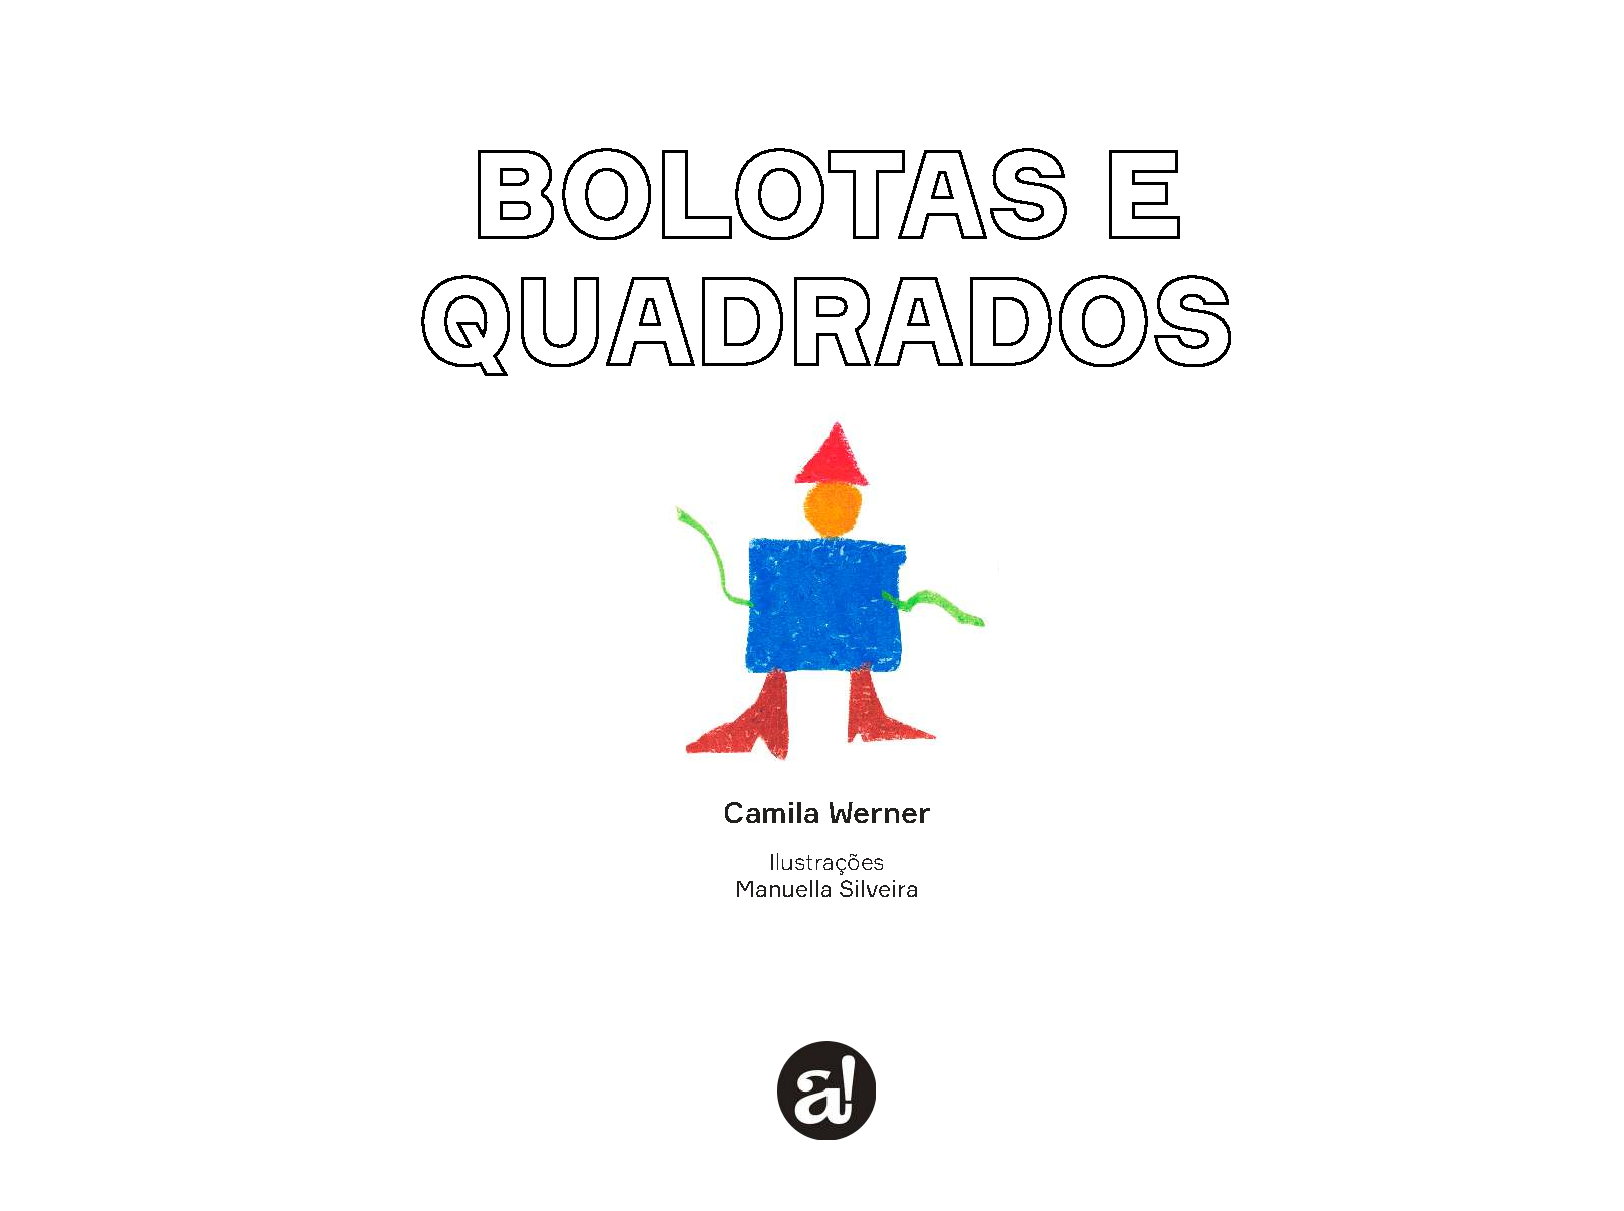
\includepdf[nup=2x2, 					% grid
			% offset=-15mm -5mm, 		% posição
			% scale=.8, 				% tamanho da página
            % delta=4mm 4mm, 			
            % frame,
            % pages={1-4}]{pdfs/PNLD2022-001_MIOLO.pdf}

\end{document}
